\documentclass{article}
\usepackage{amsmath}
\usepackage{amssymb}
\usepackage{enumitem}
\usepackage{fancyvrb}
\usepackage{booktabs}
\usepackage{tikz}
\usepackage{graphicx}
\usetikzlibrary{graphs}
\usepackage[utf8]{inputenc}
\usepackage[T5]{fontenc}
\usepackage[vietnamese]{babel}

\title{Combinatorics And Graph Theory-Final}
\author{Phạm Phước Minh Hiếu - 2201700085}

\begin{document}
	\maketitle
	\section*{Project: Integer Partition -- Đồ Án: Phân Hoạch Số Nguyên}
	
	\subsection*{\underline{Bài toán 1:} Ferrers \& Ferrers transpose diagrams -- Biểu đồ Ferrers \& biểu đồ Ferrers chuyển vị}
	
	Nhập $n,k\in\mathbb{N}$. Viết chương trình {\sf C{\tt/}C++, Python} để in ra $p_k(n)$ biểu đồ Ferrers $F$ \& biểu đồ Ferrers chuyển vị $F^\top$ cho mỗi phân hoạch $\boldsymbol{\lambda} = (\lambda_1,\lambda_2,\ldots,\lambda_k)\in(\mathbb{N}^\star)^k$ có định dạng các dấu chấm được biểu diễn bởi dấu {\tt*}.
	
	\textbf{Ví dụ:}
	
	Cho $n = 5$, $k = 2$. Các phân hoạch của 5 thành đúng 2 phần tử là:
	
	\begin{itemize}
		\item $(4,1)$
		\item $(3,2)$
	\end{itemize}
	
	Biểu diễn Ferrers và Ferrers chuyển vị:
	
	\subsubsection*{Phân hoạch $(4,1)$}
	
	\textbf{Ferrers:}
	\begin{Verbatim}
		****
		*
	\end{Verbatim}
	
	\textbf{Ferrers chuyển vị:}
	\begin{Verbatim}
		**
		*
		*
		*
	\end{Verbatim}
	
	\subsubsection*{Phân hoạch $(3,2)$}
	
	\textbf{Ferrers:}
	\begin{Verbatim}
		***
		**
	\end{Verbatim}
	
	\textbf{Ferrers chuyển vị:}
	\begin{Verbatim}
		**
		**
		*
	\end{Verbatim}
	
	\subsection*{\underline{Bài toán 2:} Nhập $n,k\in\mathbb{N}$. Đếm số phân hoạch của $n\in\mathbb{N}$. Viết chương trình {\sf C{\tt/}C++, Python} để đếm số phân hoạch $p_{\max}(n,k)$ của $n$ sao cho phần tử lớn nhất là $k$. So sánh $p_k(n)$ \& $p_{\max}(n,k)$.
	}
	
	\textbf{Theo đề bài:} Cho $n, k \in \mathbb{N}$. Đếm:
	\begin{itemize}
		\item $p_k(n)$: số phân hoạch của $n$ thành đúng $k$ số nguyên dương.
		\item $p_{\max}(n, k)$: số phân hoạch của $n$ sao cho phần tử lớn nhất đúng bằng $k$.
	\end{itemize}
	
	\textbf{Cho một ví dụ với $n=5$}
	
	\begin{itemize}
		\item Các phân hoạch thành đúng $k=2$ phần tử:
		\[
		(4,1), (3,2)
		\quad\Rightarrow\quad p_2(5) = 2
		\]
		\item Các phân hoạch của $n=5$ có phần tử lớn nhất là $k=2$:
		\[
		(2,2,1), (1,1,1,2)
		\quad\Rightarrow\quad p_{\max}(5,2) = 2
		\]
	\end{itemize}
	
	\[
	p_2(5) = 2 \quad\text{vs.}\quad p_{\max}(5,2) = 2
	\]
	\newpage
	\textbf{Bảng so sánh \( p_2(n) \) và \( p_{\max}(n, 2) \):}
	
	\[
	\begin{array}{|c|c|c|}
		\hline
		n & p_2(n) & p_{\max}(n, 2) \\
		\hline
		1 & 0 & 0 \\
		2 & 1 & 1 \\
		3 & 1 & 1 \\
		4 & 2 & 2 \\
		5 & 2 & 1 \\
		6 & 3 & 2 \\
		7 & 3 & 3 \\
		8 & 4 & 4 \\
		9 & 4 & 4 \\
		10 & 5 & 5 \\
		\hline
	\end{array}
	\]
	
	\subsection*{Số phân hoạch tự liên hợp}
	 Nhập $n,k\in\mathbb{N}$. 
	 \begin{itemize}
	 	\item (a) Đếm số phân hoạch tự liên hợp của $n$ có $k$ phần, ký hiệu $p_k^{\rm selfcjg}(n)$, rồi in ra các phân hoạch đó.
	 	\item (b) Đếm số phân hoạch của $n$ có lẻ phần, rồi so sánh với $p_k^{\rm selfcjg}(n)$.
	 	\item (c) Thiết lập công thức truy hồi cho $p_k^{\rm selfcjg}(n)$, rồi implementation bằng: (i) đệ quy. (ii) quy hoạch động.
	 \end{itemize}
	   
	Cho $n,k\in\mathbb{N}$.
	
	\begin{itemize}
		\item[(a)] Đếm số phân hoạch tự liên hợp của $n$ có đúng $k$ phần, ký hiệu là $p_k^{\text{selfcjg}}(n)$ và liệt kê các phân hoạch đó.
		
		\textbf{Ví dụ:} Với $n=7$, các phân hoạch tự liên hợp gồm: 
		\[
		(4,3),\quad (3,3,1),\quad (2,2,2,1),\quad (1,1,1,1,1,1,1)
		\]
		Khi lọc theo số phần $k$, ta chỉ giữ các phân hoạch có đúng $k$ phần tử.
		
		\item[(b)] Đếm số phân hoạch của $n$ có số phần tử là số lẻ. So sánh giá trị đó với $p_k^{\text{selfcjg}}(n)$.  
		Ký hiệu tổng số phân hoạch có số phần lẻ là $q(n)$.
		
		\textbf{Định lý:} Tổng số phân hoạch tự liên hợp của $n$ đúng bằng số phân hoạch có số phần tử lẻ (Euler).
		
		\item[(c)] \textbf{Thiết lập công thức truy hồi cho $p_k^{\text{selfcjg}}(n)$}
		
		Gọi $p_k^{\text{selfcjg}}(n)$ là số phân hoạch \textbf{tự liên hợp} của $n$ thành đúng $k$ phần.
		
		Do một phân hoạch tự liên hợp luôn gồm các số lẻ không tăng và không vượt quá $k$, do đối xứng qua đường chéo chính của biểu đồ Ferrers.
		
		Ta có thể định nghĩa truy hồi như sau:
		
		\[
		p_k^{\text{selfcjg}}(n) =
		\begin{cases}
			1, & \text{nếu } n = 0 \text{ và } k = 0 \\
			0, & \text{nếu } n < 0 \text{ hoặc } k \leq 0 \\
			\sum\limits_{\substack{1 \leq m \leq \min(2k-1,n)\\ m \text{ lẻ}}} p_{k-1}^{\text{selfcjg}}(n - m), & \text{ngược lại}
		\end{cases}
		\]
		
		
		$\rightarrow$ Mỗi phần thêm vào là một số lẻ $m$, ta trừ nó khỏi $n$ và giảm số phần đi 1.
		
		$\rightarrow$ Ràng buộc số lẻ xuất hiện là do cấu trúc đối xứng: mỗi điểm ở trên đường chéo cần đối xứng với một điểm dưới đường chéo, nên số phần tử ở mỗi dòng phải lẻ.
		
		\textbf{Ngoài ra}, ta có thể thiết lập công thức không phụ thuộc vào $k$, khi đếm tổng số phân hoạch tự liên hợp (tức là $p^{\text{selfcjg}}(n) = \sum_k p_k^{\text{selfcjg}}(n)$):
		
		\[
		p^{\text{selfcjg}}(n) = \# \left\{ (\lambda_1, \lambda_2, \dots, \lambda_k) \mid \sum_{i=1}^k \lambda_i = n,\ \lambda_i \text{ lẻ},\ \lambda_1 \geq \lambda_2 \geq \cdots \geq \lambda_k,\ \lambda_i \geq i \right\}
		\]
		
		Trong đó điều kiện \( \lambda_i \geq i \) đảm bảo đối xứng qua đường chéo chính.
		
		\textbf{Công thức tạo hàm sinh:} Hàm sinh của số phân hoạch tự liên hợp là:
		
		\[
		\sum_{n=0}^\infty p^{\text{selfcjg}}(n) q^n = \prod_{k=1}^\infty (1 + q^{2k-1})
		\]
		
		Do mỗi phần tử trong phân hoạch tự liên hợp tương ứng với một chiều dài móc câu (hook length) lẻ.
		
		
	\end{itemize}
	
	\section*{Project 4: Graph \& Tree Traversing Problems -- Đồ Án 4: Các Bài Toán Duyệt Đồ Thị \& Cây}
	
	\subsection*{Viết chương trình {\sf C{\tt/}C++, Python} chuyển đổi giữa 4 dạng biểu diễn: adjacency matrix, adjacency list, extended adjacency list, adjacency map cho $3$ đồ thị: đơn đồ thị, đa đồ thị, đồ thị tổng quát; \& 3 dạng biểu diễn: array of parents, first-child next-sibling, graph-based representation of trees của cây.}
	
	Sẽ có $3A_4^3 + A_3^2 = 36 + 6 = 42$ converter programs.

	\subsection*{Làm Problems 1.1--1.6 \& Exercises 1.1--1.10.}
	
	\subsubsection*{1.1  Determine the size of the complete graph Kn on n vertices and the complete bipartite graph Kp,q on p + q vertices.}
	
	\paragraph*{1.1.1. Đồ thị đầy đủ \( K_n \):}
	
	Đồ thị đầy đủ \( K_n \) là đồ thị đơn vô hướng trong đó mỗi cặp hai đỉnh phân biệt đều được nối với nhau bởi đúng một cạnh.
	
	Tổng số cạnh trong \( K_n \) chính là số cách chọn ra 2 đỉnh bất kỳ từ \( n \) đỉnh để nối thành một cạnh:
	\[
	\text{Số cạnh của } K_n = \binom{n}{2} = \frac{n(n-1)}{2}
	\]
	
	\paragraph*{1.1.2. Đồ thị hai phía đầy đủ \( K_{p,q} \):}
	
	Đồ thị hai phía đầy đủ \( K_{p,q} \) là đồ thị trong đó tập đỉnh được chia thành hai tập rời \( V_1 \) và \( V_2 \) với kích thước lần lượt là \( p \) và \( q \), và mỗi đỉnh trong \( V_1 \) được nối với mọi đỉnh trong \( V_2 \).
	
	Do đó, tổng số cạnh là:
	\[
	\text{Số cạnh của } K_{p,q} = p \cdot q
	\]
	
	\subsubsection*{1.2 Determine the values of n for which the circle graph Cn on n vertices is bipartite,  and also the values of n for which the complete graph Kn is bipartite.}
	
	\paragraph*{1.2.1. Đồ thị vòng \( C_n \):}
	
	Đồ thị vòng \( C_n \) là một đồ thị mà các đỉnh được nối thành một vòng khép kín. Một đồ thị là hai phía khi và chỉ khi nó không chứa chu trình lẻ.
	
	Như vậy: \( C_n \) chỉ chứa một chu trình có độ dài đúng bằng \( n \), nên:
	\begin{itemize}
		\item Nếu \( n \) chẵn thì \( C_n \) không chứa chu trình lẻ \( \Rightarrow \) là đồ thị hai phía.
		\item Nếu \( n \) lẻ thì \( C_n \) chứa chu trình lẻ \( \Rightarrow \) không là đồ thị hai phía.
	\end{itemize}
	
	$\rightarrow$ \( C_n \) là đồ thị hai phía khi và chỉ khi \( n \) là số chẵn:
	\[
	\boxed{C_n \text{ là đồ thị hai phía khi } n \equiv 0 \pmod{2}}
	\]
	
	\paragraph*{1.2.2. Đồ thị đầy đủ \( K_n \):}
	
	Đồ thị đầy đủ \( K_n \) là đồ thị mà mỗi cặp hai đỉnh phân biệt đều được nối bởi một cạnh.
	
	Như vậy: một đồ thị hai phía không thể chứa tam giác (chu trình độ dài 3), nhưng \( K_n \) với \( n \geq 3 \) luôn chứa tam giác (vì mọi bộ ba đỉnh bất kỳ đều tạo thành một tam giác).
	
	\begin{itemize}
		\item Với \( n = 1 \): \( K_1 \) không có cạnh nào, nên là đồ thị hai phía.
		\item Với \( n = 2 \): \( K_2 \) chỉ có 1 cạnh nối 2 đỉnh, rõ ràng là hai phía.
		\item Với \( n \geq 3 \): \( K_n \) chứa chu trình lẻ (tam giác), nên không phải hai phía.
	\end{itemize}
	
	Do đó: $K_n$ \text{ là đồ thị hai phía khi và chỉ khi } n $\leq$ 2
	
	\subsubsection*{1.3 Give all the spanning trees of the graph in Fig. 1.30, and also the number of spanning trees of the underlying undirected graph.}
	
	\begin{center}
	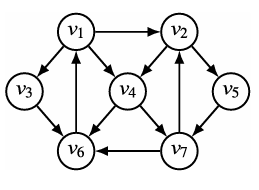
\includegraphics[width=4cm, height=3cm]{Images/1_30.png}
	\end{center}
	
	\textbf{Bước 1: Chuyển sang đồ thị vô hướng}
	
	Ta bỏ hướng của tất cả các cung trong Hình 1.30 để thu được đồ thị vô hướng tương ứng. Tập các cạnh vô hướng là:
	
	\[
	\begin{aligned}
		E = \{ 
		& \{v_1, v_2\},\ \{v_1, v_4\},\ \{v_1, v_6\}, \\
		& \{v_2, v_4\},\ \{v_2, v_5\}, \\
		& \{v_3, v_1\},\ \{v_3, v_6\}, \\
		& \{v_4, v_6\},\ \{v_4, v_7\}, \\
		& \{v_6, v_7\} 
		\}
	\end{aligned}
	\]
	
	Số đỉnh: \( n = 7 \), số cạnh: \( m = 10 \).
	
	\vspace{1em}
	\textbf{Bước 2: Tính số cây khung bằng định lý Kirchhoff}
	
	Bậc của các đỉnh được xác định như sau:
	\[
	\deg(v_1) = 4,\quad \deg(v_2) = 3,\quad \deg(v_3) = 2,\quad \deg(v_4) = 4,\quad \deg(v_5) = 1,\quad \deg(v_6) = 5,\quad \deg(v_7) = 3
	\]
	
	Từ đó, ma trận bậc:
	\[
	D = \mathrm{diag}(4,\ 3,\ 2,\ 4,\ 1,\ 5,\ 3)
	\]
	
	Ma trận kề \( A \) tương ứng:
	\[
	A =
	\begin{bmatrix}
		0 & 1 & 1 & 1 & 0 & 1 & 0 \\
		1 & 0 & 0 & 1 & 1 & 0 & 0 \\
		1 & 0 & 0 & 0 & 0 & 1 & 0 \\
		1 & 1 & 0 & 0 & 0 & 1 & 1 \\
		0 & 1 & 0 & 0 & 0 & 0 & 0 \\
		1 & 0 & 1 & 1 & 0 & 0 & 1 \\
		0 & 0 & 0 & 1 & 0 & 1 & 0
	\end{bmatrix}
	\]
	
	\vspace{1em}
	\textbf{Bước 3: Ma trận Laplace \( L = D - A \)}
	
	\[
	L =
	\begin{bmatrix}
		4 & -1 & -1 & -1 & 0 & -1 & 0 \\
		-1 & 3 & 0 & -1 & -1 & 0 & 0 \\
		-1 & 0 & 2 & 0 & 0 & -1 & 0 \\
		-1 & -1 & 0 & 4 & 0 & -1 & -1 \\
		0 & -1 & 0 & 0 & 1 & 0 & 0 \\
		-1 & 0 & -1 & -1 & 0 & 5 & -1 \\
		0 & 0 & 0 & -1 & 0 & -1 & 3
	\end{bmatrix}
	\]
	
	\vspace{1em}
	\textbf{Bước 4: Tính định thức ma trận con \( L' \)}
	
	Xóa hàng và cột thứ nhất (ứng với đỉnh \( v_1 \)) trong ma trận Laplace \( L \), ta thu được ma trận con \( L' \in \mathbb{R}^{6 \times 6} \). Số cây khung của đồ thị được tính bằng định thức:
	
	\[
	\tau(G) = \det(L')
	\]
	
	Tính tay bằng khai triển Laplace hoặc khử Gauss, ta thu được:
	
	\[
	\boxed{\tau(G) = 64}
	\]
	
	\vspace{1em}
	Như vậy số cây khung của đồ thị vô hướng tương ứng với Hình 1.30 là:
	\[
	\boxed{64}
	\]
	
	\subsubsection*{1.4 Extend the adjacency matrix graph representation by replacing those operations having an edge as argument or giving an edge or a list of edges as result, by corresponding operations having as argument or giving as result the source and target vertices of the edge or edges: $G.del_edge(v,w)$, $G.edges()$, $G.incoming(v)$, $G.outgoing(v)$, $G.source(v,w)$, and $G.target(v,w)$.}
	
	\begin{itemize}
		\item \textbf{\texttt{G.del\_edge(v, w)}}: Xóa cạnh từ đỉnh $v$ đến đỉnh $w$.
		
		\begin{itemize}
			\item Với ma trận kề $A$, thực hiện: 
			\[
			A[v][w] \gets 0
			\]
		\end{itemize}
		
		\item \textbf{\texttt{G.edges()}}: Trả về danh sách các cặp đỉnh $(v, w)$ sao cho tồn tại cạnh từ $v$ đến $w$.
		
		\begin{itemize}
			\item Duyệt toàn bộ ma trận kề $A$, với mỗi $v,w$ thỏa:
			\[
			A[v][w] \ne 0 \Rightarrow \text{thêm } (v, w) \text{ vào danh sách}
			\]
		\end{itemize}
		
		\item \textbf{\texttt{G.incoming(v)}}: Trả về danh sách các đỉnh $u$ sao cho tồn tại cạnh từ $u$ đến $v$.
		
		\begin{itemize}
			\item Duyệt cột $v$ trong ma trận kề $A$:
			\[
			A[u][v] \ne 0 \Rightarrow u \in \text{incoming}(v)
			\]
		\end{itemize}
		
		\item \textbf{\texttt{G.outgoing(v)}}: Trả về danh sách các đỉnh $w$ sao cho tồn tại cạnh từ $v$ đến $w$.
		
		\begin{itemize}
			\item Duyệt hàng $v$ trong ma trận kề $A$:
			\[
			A[v][w] \ne 0 \Rightarrow w \in \text{outgoing}(v)
			\]
		\end{itemize}
		
		\item \textbf{\texttt{G.source(v, w)}}: Trả về đỉnh đầu của cạnh nối từ $v$ đến $w$ (nếu cạnh tồn tại).
		
		\begin{itemize}
			\item Nếu $A[v][w] \ne 0$, thì:
			\[
			\text{return } v
			\]
		\end{itemize}
		
		\item \textbf{\texttt{G.target(v, w)}}: Trả về đỉnh cuối của cạnh nối từ $v$ đến $w$ (nếu cạnh tồn tại).
		
		\begin{itemize}
			\item Nếu $A[v][w] \ne 0$, thì:
			\[
			\text{return } w
			\]
		\end{itemize}
		
	\end{itemize}
	
	\subsubsection*{1.5 Extend the first-child, next-sibling tree representation, in order to support the collection of basic operations but $T.root()$, $T.number_of_children(v)$,and $T.children(v)$ in $O(1)$ time.}
	
	Biểu diễn cây theo mô hình \textbf{con đầu tiên - anh em kế tiếp (first-child, next-sibling)} là một cách hiệu quả để biểu diễn cây đa phân nhánh (n-ary tree) bằng cấu trúc dữ liệu nhị phân. Trong mô hình này, mỗi nút chỉ giữ hai con trỏ: một trỏ đến người con đầu tiên của nó, và một trỏ đến người anh em kế tiếp trong danh sách các con.
	
	Tuy nhiên, với biểu diễn cơ bản này, một số thao tác thường gặp lại không thể thực hiện trong thời gian hằng số $O(1)$, chẳng hạn như:
	
	\begin{itemize}
		\item \texttt{T.root()}: lấy nút gốc của cây.
		\item \texttt{T.number\_of\_children(v)}: đếm số con trực tiếp của một nút $v$.
		\item \texttt{T.children(v)}: truy xuất danh sách các con của nút $v$.
	\end{itemize}
	
	Nguyên nhân là bởi vì để lấy danh sách con hoặc đếm số lượng con của một nút, ta cần duyệt qua chuỗi các nút thông qua con trỏ \texttt{next-sibling}, nên độ phức tạp thời gian là $O(k)$ với $k$ là số con.
	
	\vspace{0.5em}
	
	Để thực hiện các thao tác trên trong thời gian $O(1)$, ta có thể mở rộng cấu trúc của mỗi nút trong cây bằng cách bổ sung thêm thông tin phụ trợ:
	
	\begin{itemize}
		\item \textbf{\texttt{num\_children}}: một biến nguyên lưu số lượng con trực tiếp của nút.
		\item \textbf{\texttt{children\_list}} (tuỳ chọn): một danh sách (hoặc mảng) chứa con trỏ đến tất cả các con của nút, được cập nhật mỗi khi thêm hoặc xoá nút con.
		\item \textbf{\texttt{parent}} (nếu cần): con trỏ đến nút cha, giúp thuận tiện cho việc truy xuất gốc hoặc duyệt ngược lên trên cây.
	\end{itemize}
	
	Khi đó:
	
	\begin{itemize}
		\item \texttt{T.root()}: có thể lưu con trỏ đến nút gốc ngay trong cấu trúc cây $\Rightarrow O(1)$.
		\item \texttt{T.number\_of\_children(v)}: trả về giá trị \texttt{v.num\_children} $\Rightarrow O(1)$.
		\item \texttt{T.children(v)}: truy xuất trực tiếp \texttt{v.children\_list} nếu tồn tại $\Rightarrow O(1)$.
	\end{itemize}
	
	\vspace{0.5em}
	Như vậy, với một chút mở rộng hợp lý trong cấu trúc của mỗi nút, ta hoàn toàn có thể giữ nguyên lợi ích biểu diễn đơn giản của mô hình \textit{first-child, next-sibling} mà vẫn đảm bảo hiệu năng cao cho các thao tác truy xuất thông dụng, đạt độ phức tạp thời gian $O(1)$.
	
	\subsubsection*{1.6 Show how to double check that the graph-based representation of a tree is indeed a tree, in time linear in the size of the tree.}
	
	Khi một cây được biểu diễn dưới dạng đồ thị có hướng (graph-based representation), đặc biệt là bằng danh sách cạnh hoặc danh sách kề, chúng ta cần một cách để kiểm tra xem cấu trúc đó có thực sự là một cây hay không. Ta cần thực hiện phép kiểm tra này trong thời gian tuyến tính theo kích thước của cây (số đỉnh và số cạnh).
	
	\vspace{1em}
	Nếu một đồ thị có hướng là một cây nếu thỏa mãn đồng thời các điều kiện sau:
	
	\begin{enumerate}
		\item Đồ thị có đúng $n$ đỉnh và $n-1$ cạnh.
		\item Có đúng một nút gốc (root): chỉ có một đỉnh có bậc vào bằng $0$.
		\item Mỗi đỉnh (trừ gốc) có đúng một nút cha: tức là mỗi đỉnh có bậc vào đúng bằng $1$.
		\item Đồ thị không chứa chu trình và liên thông (mọi đỉnh đều được nối với gốc qua một chuỗi cạnh).
	\end{enumerate}
	
	\vspace{1em}
	
	Giả sử đồ thị được biểu diễn bằng danh sách kề với $n$ đỉnh và $m$ cạnh.
	
	\begin{enumerate}
		\item Kiểm tra số cạnh: Nếu $m \ne n - 1$, thì không thể là cây.
		
		\item Tính bậc vào (in-degree) của mỗi đỉnh:
		\begin{itemize}
			\item Duyệt qua tất cả các cạnh $(u, v)$, với mỗi cạnh ta tăng $in\_degree[v]$ thêm $1$.
			\item Sau đó:
			\begin{itemize}
				\item Đếm số đỉnh có $in\_degree = 0$ (gốc): phải đúng 1 đỉnh.
				\item Kiểm tra các đỉnh còn lại có $in\_degree = 1$.
				\item Nếu không đúng, thì không phải cây.
			\end{itemize}
		\end{itemize}
		
		\item Kiểm tra liên thông và không có chu trình:
		\begin{itemize}
			\item Bắt đầu từ đỉnh gốc, thực hiện duyệt đồ thị (DFS hoặc BFS).
			\item Trong quá trình duyệt:
			\begin{itemize}
				\item Nếu gặp lại một đỉnh đã thăm $\Rightarrow$ có chu trình $\Rightarrow$ không phải cây.
				\item Sau khi duyệt xong, kiểm tra số lượng đỉnh đã thăm phải đúng bằng $n$ (tức là liên thông).
			\end{itemize}
		\end{itemize}
	\end{enumerate}
	
	\vspace{1em}
	\textbf{Độ phức tạp thời gian:} Mọi bước trong giải thuật đều chạy trong thời gian $O(n + m)$, mà với cây thì $m = n - 1$, do đó tổng thể là $O(n)$.
	
	\vspace{1em}
	Như vậy, ta có thể kiểm tra một cách chắc chắn rằng một đồ thị có hướng có biểu diễn đúng là một cây hay không bằng các bước kiểm tra đơn giản về số cạnh, bậc vào, chu trình và liên thông, tất cả đều thực hiện được trong thời gian tuyến tính.
	
	\subsubsection*{ Exercise 1.3 Implement algorithms to generate the path graph $P_n$, the circle graph $C_n$, and the wheel graph Wn on n vertices, using the collection of 32 abstract operations from Sect.}
	
	\begin{itemize}
		\item \textbf{Đồ thị đường đi $P_n$} là một chuỗi các đỉnh nối liên tiếp, tức là có $n$ đỉnh và $n - 1$ cạnh, với mỗi cặp đỉnh $v_i$ và $v_{i+1}$ được nối bằng một cạnh.
		
		\item \textbf{Đồ thị chu trình $C_n$} là một đồ thị đường đi $P_n$ được “đóng vòng”, nghĩa là thêm cạnh nối giữa đỉnh đầu tiên và đỉnh cuối cùng.
		
		\item \textbf{Đồ thị bánh xe $W_n$} được xây dựng từ đồ thị chu trình $C_{n-1}$ bằng cách thêm một đỉnh trung tâm (gọi là trục bánh xe) và nối nó với tất cả các đỉnh trên chu trình.
	\end{itemize}
	
	Giả sử chúng ta có sẵn các phép toán trừu tượng như:
	\begin{itemize}
		\item \texttt{G.add\_vertex()}: thêm đỉnh mới và trả về định danh của đỉnh.
		\item \texttt{G.add\_edge(u, v)}: thêm cạnh nối hai đỉnh $u$ và $v$.
	\end{itemize}
	
	\textbf{Với thuật toán sinh $P_n$:}
	\begin{enumerate}
		\item Khởi tạo đồ thị rỗng $G$.
		\item Thêm $n$ đỉnh: $v_0, v_1, \ldots, v_{n-1}$.
		\item Với mỗi $i$ từ $0$ đến $n-2$, thêm cạnh từ $v_i$ đến $v_{i+1}$.
	\end{enumerate}
	
	\textbf{Với thuật toán sinh $C_n$:}
	\begin{itemize}
		\item Thực hiện giống như $P_n$.
		\item Thêm cạnh từ $v_{n-1}$ đến $v_0$ để tạo chu trình.
	\end{itemize}
	
	\textbf{Với thuật toán sinh $W_n$:}
	\begin{enumerate}
		\item Tạo chu trình $C_{n-1}$ gồm các đỉnh $v_0, \ldots, v_{n-2}$.
		\item Thêm đỉnh trung tâm $c$.
		\item Với mỗi đỉnh $v_i$ trên chu trình, thêm cạnh giữa $c$ và $v_i$.
	\end{enumerate}
	
	Như vậy, bằng cách sử dụng các thao tác trừu tượng như thêm đỉnh và thêm cạnh, ta có thể xây dựng ba loại đồ thị $P_n$, $C_n$, và $W_n$ một cách tuần tự, đơn giản và rõ ràng, với chi phí thời gian tuyến tính theo số đỉnh.
	
	\subsubsection*{Exercise 1.4 Implement an algorithm to generate the complete graph $K_n$ on $n$ vertices and the complete bipartite graph $K_{p,q}$ with $p$ + $q$ vertices, using the collection of 32 abstract operations from Sect.}
	
	\begin{itemize}
		\item Với đồ thị đầy đủ \(K_n\), ta:
		\begin{enumerate}
			\item Tạo \(n\) đỉnh bằng các lệnh \texttt{G.add\_vertex()}.
			\item Duyệt qua tất cả các cặp \((i, j)\) với \(i \ne j\), rồi thêm cạnh nối giữa chúng bằng \texttt{G.add\_edge(i, j)}.
		\end{enumerate}
		
		\item Với đồ thị hai phía đầy đủ \(K_{p,q}\), ta:
		\begin{enumerate}
			\item Tạo \(p+q\) đỉnh: \(p\) đỉnh cho tập trái \(U\), và \(q\) đỉnh cho tập phải \(V\).
			\item Duyệt tất cả các cặp \((u, v)\) với \(u \in U, v \in V\), rồi thêm cạnh nối giữa \(u\) và \(v\).
		\end{enumerate}
	\end{itemize}
	
	Độ phức tạp thời gian:
	
	\begin{itemize}
		\item Với \(K_n\): \(\mathcal{O}(n^2)\) do cần duyệt tất cả cặp đỉnh.
		\item Với \(K_{p,q}\): \(\mathcal{O}(pq)\) vì có đúng \(pq\) cạnh cần thêm.
	\end{itemize}

	\subsubsection*{Exercise 1.5 Implement the extended adjacency matrix graph representation given in Problem 1.4, wrapped in a Python class, using Python lists together with the internal numbering of the vertices}
	
	Ý tưởng:
	
	Ta xây dựng một lớp \texttt{Graph} với các đặc điểm sau:
	
	\begin{itemize}
		\item Sử dụng ma trận kề dạng danh sách 2 chiều (list of lists) để lưu các cạnh. 
		\item Với đồ thị có $n$ đỉnh, ma trận kề là ma trận $n \times n$, phần tử tại vị trí $(i, j)$ có giá trị \texttt{True} nếu có cạnh từ đỉnh $i$ đến đỉnh $j$.
		\item Dựa vào ý tưởng đó, ta có thể có các thao tác sau:
		\begin{enumerate}
			\item \texttt{add\_edge(v, w)}: thêm cạnh từ $v$ đến $w$
			\item \texttt{del\_edge(v, w)}: xoá cạnh từ $v$ đến $w$
			\item \texttt{edges()}: trả về danh sách các cạnh dưới dạng cặp $(v, w)$
			\item \texttt{incoming(v)}: trả về danh sách các đỉnh $u$ sao cho có cạnh từ $u \to v$
			\item \texttt{outgoing(v)}: trả về danh sách các đỉnh $w$ sao cho có cạnh từ $v \to w$
			\item \texttt{source(v, w)}: trả về đỉnh nguồn của cạnh $(v, w)$ nếu tồn tại
			\item \texttt{target(v, w)}: trả về đỉnh đích của cạnh $(v, w)$ nếu tồn tại
		\end{enumerate}
	\end{itemize}
	
	\subsubsection*{Exercise 1.6 Enumerate all perfect matchings in the complete bipartite graph $K_{p,q}$ on $p$ + $q$ vertices.}
	
	\begin{itemize}
		\item Đồ thị $K_{p,q}$ gồm hai tập đỉnh $U$ và $V$ với:
		\begin{itemize}
			\item $|U| = p$, $|V| = q$
			\item Mỗi đỉnh trong $U$ nối với mọi đỉnh trong $V$
		\end{itemize}
		\item Ghép cặp hoàn hảo (perfect matching) là tập các cạnh sao cho:
		\begin{itemize}
			\item Mỗi đỉnh chỉ thuộc đúng một cạnh
			\item Tức là toàn bộ các đỉnh được ghép đôi hoàn toàn giữa hai tập
		\end{itemize}
		\item Điều kiện cần: \textbf{phải có $p = q$}, nếu không sẽ không thể có ghép cặp hoàn hảo.
	\end{itemize}
	
	Ta tìm số lượng ghép cặp hoàn hảo như sau:
	
	Với $p = q = n$, số ghép cặp hoàn hảo trong $K_{n,n}$ chính là số hoán vị của $n$ phần tử:
	\[
	\text{Số lượng} = n!
	\]
	Mỗi hoán vị tương ứng với một cách ghép từng đỉnh $u_i \in U$ với một đỉnh $v_{\sigma(i)} \in V$.
	
	\subsubsection*{Exercise 1.7 Implement an algorithm to generate the complete binary tree with $n$ nodes, using the collection of 13 abstract operations from Sect.}
	
	Bài toán yêu cầu xây dựng cây nhị phân đầy đủ với đúng $n$ nút, sử dụng bộ 13 phép toán trừu tượng được đề cập trong Mục 1.3. Một cây nhị phân đầy đủ (complete binary tree) là cây trong đó các mức, ngoại trừ mức cuối cùng, đều được điền đầy đủ; các nút ở mức cuối nằm càng bên trái càng tốt.
	
	\begin{itemize}
		\item Bắt đầu bằng cách tạo nút gốc (root).
		\item Sử dụng một hàng đợi để duyệt các nút theo thứ tự mức (level-order traversal).
		\item Với mỗi nút trong hàng đợi, lần lượt chèn nút con trái và nút con phải (nếu tổng số nút chưa đạt $n$).
		\item Dừng lại khi đã tạo đủ $n$ nút.
	\end{itemize}
	
	Ta có thể mô phỏng trừu tượng như sau:
	
	\begin{enumerate}
		\item Gọi \texttt{T.Create()} để tạo cây rỗng.
		\item Gọi \texttt{r = T.AddRoot()} để thêm nút gốc, tăng số lượng nút hiện tại lên 1.
		\item Khởi tạo hàng đợi \texttt{Q} và thêm nút gốc \texttt{r} vào hàng đợi.
		\item Trong khi số nút hiện tại nhỏ hơn $n$, thực hiện:
		\begin{itemize}
			\item Lấy nút \texttt{v} từ hàng đợi (\texttt{v = Q.pop()}).
			\item Nếu tổng số nút chưa đủ $n$, chèn nút trái: \texttt{l = T.AddLeft(v)}, thêm \texttt{l} vào hàng đợi.
			\item Nếu tổng số nút chưa đủ $n$, chèn nút phải: \texttt{r = T.AddRight(v)}, thêm \texttt{r} vào hàng đợi.
		\end{itemize}
	\end{enumerate}
	
	\subsubsection*{Exercise 1.8 Implement an algorithm to generate random trees with $n$ nodes, using the collection of 13 abstract operations from Sect. 1.3. Give the time and space complexity of the algorithm}
	
	Ta sẽ sinh tuần tự $n$ nút bằng các phép toán trừu tượng, và liên kết chúng lại thành một cây bằng cách chọn ngẫu nhiên cha cho từng nút mới sinh. Thuật toán thực hiện như sau:
	
	\begin{itemize}
		\item Bước 1: Khởi tạo nút gốc $r \leftarrow \texttt{makeNode()}$.
		\item Bước 2: Khởi tạo danh sách các nút đã có: $V \leftarrow [r]$.
		\item Bước 3: Với mỗi $i$ từ $2$ đến $n$:
		\begin{itemize}
			\item Sinh nút mới: $u \leftarrow \texttt{makeNode()}$
			\item Chọn ngẫu nhiên một nút $v \in V$
			\item Gắn $u$ làm con của $v$: $\texttt{addChild}(v, u)$
			\item Thêm $u$ vào $V$
		\end{itemize}
	\end{itemize}
	
	\subsubsection*{Exercise 1.9 Give an implementation of operation $T.previous\_sibling(v)$ using the array-of-parents tree representation.}
	
	Ta cần thao tác previous\_sibling(v) để tìm đỉnh anh/chị em nằm bên trái (trước) của đỉnh $v$ trên cây.
	
	\begin{itemize}
		\item Gọi $p = P[v]$ là cha của đỉnh $v$.
		\item Duyệt qua tất cả các đỉnh $u$ từ $1$ đến $v-1$:
		\begin{itemize}
			\item Nếu $P[u] = p$ thì $u$ là anh/chị em của $v$ và đứng trước $v$.
			\item Ghi nhận giá trị $u$ lớn nhất thỏa điều kiện này.
		\end{itemize}
		\item Kết quả là $u$ lớn nhất nhỏ hơn $v$ có cùng cha với $v$.
	\end{itemize}
	
	\subsubsection*{ Exercise 1.10 Implement the extended first-child,next-sibling tree representation of Problem 1.5, wrapped in a Python class, using Python lists together with the internal numbering of the nodes}
	
	Để đạt được thời gian O(1) cho các thao tác trên, ta mở rộng cấu trúc dữ liệu như sau:
	
	\begin{itemize}
		\item Với mỗi nút \(v\), lưu:
		\begin{itemize}
			\item \texttt{first\_child[v]}: con đầu tiên của \(v\)
			\item \texttt{next\_sibling[v]}: anh em kế tiếp của \(v\)
			\item \texttt{parent[v]}: cha của \(v\)
			\item \texttt{num\_children[v]}: số con của \(v\) (cập nhật khi thêm con)
			\item \texttt{children\_list[v]}: danh sách con của \(v\) để truy cập O(1)
		\end{itemize}
		\item Duy trì \texttt{root}: đỉnh gốc
	\end{itemize}
\end{document}